\chapter{Vision-Based Motion Primitives for Humanoid Walking} 
\label{Chap:Visual-Planning}

In the last chapter we presented an scheme to control a humanoid robot directly by using visual servoing techniques. However, the trajectories realized by the robot in that case are generated to minimize the distance in the image feature space and might create unnecessary motion in the space of the footprints. This is because visual servoing is a local control technique. If we want to take into account the shape of the trajectory or obtacles avoidance, a planning method would be necessary.

Motion planning aims to take the robot from a initial to a final position while ensuring feasibility and obstacle avoidance. The notion of optimality arises in motion planning. From the work of \citep{Salaris:2010, jib-IJHR2010} it exists a set of optimal trajectories to take a nonholonomic robot from a initial to a final position while keeping insight a landmark. It has been shown that the human walking behaves nonholonomic for long distances. In this chapter, we will work upon those works and we will inject the motion primitives from the planner into the pattern generator level of the robot.

\section{Global planning with visibility constraints}
%==================================================================

\label{sec:globalplanning}

For visual servoing, localization, surveillance, or any robotic task based on the observation of visual cues, it is important to ensure that the robot under control does not lose sight of the landmark(s) used as a visual reference. Hence, several works have been proposed to provide motion planners that guarantee landmark visibility, mainly for wheeled robots.

With this concern in mind, we borrow one such global planner, described in~\cite{jib-IJHR2010},  as a base tool for generating paths that guarantee to enforce the required visual constraints while giving locally optimal trajectories in distance. This base planner for humanoid robots uses as an underlying model of motion, a disk-shaped non-holonomic Differential Drive Robot (DDR). In~\cite{jib-IJHR2010}, if a solution path is found for the DDR, it is converted into a solution path for the humanoid robot by generating a footprints sequence coherent with the humanoid dimensions. A nice property inherited from using the DDR model of motion is that the global planner is complete, i.e.  if a solution exists, it will give one, otherwise, it will say so.

However, even if, locally, the used motion primitives are optimal in distance, this approach does not necessarily give globally optimal trajectories. We will not detail the complete methodology here, but we recall the basic results hereafter.

The aforementioned algorithm takes as an input a 2D map of the environment, with its obstacles and visual landmarks, an initial configuration of the robot in the plane, $(x_A,y_A,\theta_A)$, and a final (goal) configuration in the plane, $(x_B,y_B,\theta_B)$. Its output is a set of footprints in the plane to be followed by the robot. The building of this path follows a classical recursive strategy: A roadmap is built over the free space, which includes both, points free of collision with the obstacles in the environment and points that are not within the shadows cast by the landmarks. Then, the initial and final configurations are tested, to check whether the optimal primitives of~\cite{Salaris:2010} can connect them without colliding forbidden regions. If the computed path is without collision, then the algorithm ends, otherwise the holonomic shortest path on the roadmap from the initial configuration to the final (if it exists) is divided in two parts by its middle point, and the whole process is repeated on the two sub-parts. 

The resulting path is made of several parts, each one corresponding to a locally optimal path given from~\cite{Salaris:2010} (made of a combination of straight lines, logarithmic spirals and in-site rotations). This allows to define a set of $S$ sub-segments to be performed by the robot along locally optimal paths, which will be referred to as $(p^s,q^s)$, for $s=1\dots S$~:
$$
p^s = (x_p^s,y_p^s,\theta_p^s)^T \; ; \; q^s = (x_q^s,y_q^s,\theta_q^s)^T,
$$

with $p^s$ the initial configuration and $q^s$ the final one. The complete computed path is executed by reaching the successive sub-goals $q^s$.


%==================================================================
\section{Defining a local reference trajectory}
%==================================================================

\label{sec:reftrajectories}

Let us focus on the execution of each sub-path $s$. Suppose that we start with the robot at some configuration close to $p^s$ (see Fig.~\ref{fig:paths}), because localization may not be perfect, and suppose that we want to reach the final configuration or sub-goal $q^s$, as determined in~\cite{jib-IJHR2010}.

\subsection{Adapting the reference trajectory for the MPC}

Without loss of generality, we suppose that the object of interest to be kept at sight by the robot is located at $\mathbf L^s = (0,0)$. In all the following, $x,y,\theta$ will refer to coordinates w.r.t a global frame centered at this origin.

It is noteworthy that, given the sub-goal $q^s =(x_q^s,y_q^s,\theta_q^s)^T$ to reach, and the landmark it is associated to, the work of~\cite{Salaris:2010} gives us a full synthesis of optimal paths in free space. This synthesis can be represented as a mapping $\sigma$:
$$
\begin{array}{cccccc}
\sigma & : & \mathbb{R}^2 & \mapsto & \mathbb{S}^1 \times \mathbb{R}^2\\
& & (x,y) & \rightarrow & (\theta^*(x,y),v^*(x,y),\omega^*(x,y))
\end{array}
$$

where $\theta^*(x,y)$ is the orientation the robot (viewed as a nonholonomic cart)  should have in order to start walking along the shortest path to $q^s$, from its current position $(x,y)$. The pair $(v^*(x,y),\omega^*(x,y))$ are the instantaneous (reference) velocities needed to be applied to follow the shortest paths. Without loss of generality, we can suppose that $v^*(x,y)=0$ (for in-site rotations) or $v^*(x,y)=\pm 1$ (elsewhere). Given the linear velocity $v^*(x,y)$, $\omega^*(x,y)$ is defined in function of the nature  of the path segment,
$$
\left\{
\begin{array}{cccc}
 \omega^*(x,y) & = & 0 & \mbox{(straight line)}\\
  & = & \pm\frac{\sin(\phi_{max})}{\sqrt{x^2+y^2}} & \mbox{(spiral)},\\
\end{array}
\right.
$$

where $\phi_{max}$ is the maximal bearing angle possible for the landmark, given the sensor and robot characteristics.

Our claim is that the knowledge of optimal policies at each point allows some flexibility when generating a walking pattern, by optimizing the footprint positions and  the CoM trajectory ``around'' the nominal path output from the planner, by using these policies within the pattern generation.

\begin{figure}[h]
\centering
 \subimport*{Chap5-Visual-Planning/}
                   {config.pdf_t}
\caption{From a configuration $(x,y,\theta)$ and its corresponding position $(x,y)$, and a sub-goal $q^s= (x_q^s,y_q^s,\theta_q^s)$ to reach, the optimal path (dashed line) is the one we want the humanoid robot to follow. For that, we use the tangent orientation $\theta^*(x,y)$ to this path. Because of the errors in control or localization, this optimal path may be different from the shortest path (solid line) computed from the first configuration $p^s= (x_p^s,y_p^s,\theta_p^s)$.
%For the linearization purposes, and given that $(x,y)$ will be variable, we will use a nominal shortest path (solid line) from a close, fixed configuration $p^s= (x_p^s,y_p^s,\theta_p^s)$.
\label{fig:paths}}
\end{figure}

In pattern generation algorithms such as~\cite{HerdtAR2010}, the cost function within the Model Predictive Control (MPC) window uses the configurations of the CoM. Here, focusing more specifically on the $(x,y,\theta)$ CoM coordinates, we handle as an input of the algorithm a reference trajectory to be followed, and a synthesis of shortest paths leading to a given objective, as a direct output from~\cite{Salaris:2010}. As depicted in Fig.~\ref{fig:paths}, at each configuration evaluated within the MPC, two forces should apply through the optimization scheme: one driving the robot to the ``correct'' orientation $\theta^*(x,y)$, and one making the velocities follow the shortest path, $(v(x,y),\omega(x,y))$. Also, a strong visibility constraint should apply, to ensure the object of interest to stay visible. In Fig.~\ref{fig:fieldNoLateral}, we give an illustration of the shortest paths synthesis from~\cite{Salaris:2010}, displayed through the local orientations of optimal paths at each point of the plane, given the objective to reach (``end point'') and the landmark to keep in sight. 


%==================================================================
%\subsection{Tracking a single reference trajectory}
%==================================================================

%\label{subsection-singleref}

%In that case, we would track the reference path from $p^s$ to $q^s$; this has the advantage of being rather simple to express, I believe. Consider the reference path from $p^s$ to $q^s$; generate a corresponding sampled trajectory  $x_{ref}(k\tau),y_{ref}(k\tau),\theta_{ref}(k\tau)$, then stack them into vectors $C^x_{ref},C^y_{ref},C^\theta_{ref}$. Note that from the same analysis, we could also reinforce the tracking of the desired trajectories by including reference velocities, 

%$$
%\left\{
%\begin{array}{ccc}
%\dot{x}_{ref}(k\tau) & = & v \cos(\theta_{ref}(k\tau)) \\
%\dot{y}_{ref}(k\tau) & = & v \sin(\theta_{ref}(k\tau)) \\
%\dot{\theta}_{ref}(k\tau) & = & \omega(v,x_{ref}(k\tau),y_{ref}(k\tau)) \\
%\end{array}
%\right.
%$$

%where $v$ is a reference linear velocity, and $\omega(v,x_{ref}(k\tau),y_{ref}(k\tau))$ directly deduced from the synthesis. Similarly to positions, these references velocities could be stacked into $\dot{C}^x_{ref},\dot{C}^y_{ref},\dot{C}^\theta_{ref}$.

%We would introduce directly this desired trajectory in the pattern generator, while keeping the decoupled formulation of~\cite{HerdtIROS2010}, for the $x,y$ position on the one hand, and for the $\theta$ angle, on the other. Hence,

%{\small
%\begin{eqnarray}
%\nonumber
% \min && \dfrac{\alpha}{2} \left\| C^x_{i+1} - C^x_{ref} \right\|^2 + \dfrac{\alpha}{2} \left\| C^y_{i+1} - C^y_{ref} \right\|^2 \\
%\nonumber
%&& + \dfrac{\beta}{2} \left\| \dot{C}^x_{i+1} - \dot{C}^x_{ref} \right\|^2 + \dfrac{\beta}{2} \left\| \dot{C}^y_{i+1} - \dot{C}^y_{ref} \right\|^2 \\
%\nonumber
%&& + \dfrac{\gamma}{2} \left\| F^x_{i+1} - Z^x_{i+1} \right\|^2 + \dfrac{\gamma}{2} \left\| F^y_{i+1} - Z^y_{i+1} \right\|^2 \\
%&& + \dfrac{\epsilon}{2} \left\| \dddot{C}^x_{i} \right\|^2 + \dfrac{\epsilon}{2} \left\| \dddot{C}^y_{i} \right\|^2,
%\end{eqnarray}
%}

%and for the angular position,

%{\small
%\begin{eqnarray}
%\nonumber
% \min && \dfrac{\alpha}{2} \left\| C^{\theta}_{i+1} - C^{\theta}_{ref} \right\|^2 + \dfrac{\beta}{2} \left\| \dot{C}^{\theta}_{i+1} - \dot{C}^{\theta}_{ref} \right\|^2 \\
%&& \dfrac{\gamma}{2} \left\| \sum (f^{\theta}_i - c^{\theta}_i) \right\|^2 
%\label{eq-opt-orientations}
%\end{eqnarray}
%}

%where $C^{\alpha}_{ref}$ with $\alpha \in \{x,y,\theta\}$ is the reference trajectory in the horizon, extracted from the trajectory generated with the planner \cite{HayetIJHR2010}.

%Note that the same process can be applied by considering, instead of $p^s$, the point corresponding to the current robot position. This would be a first, cheap way to adapt the reference trajectory. In both cases, the orientations would have been computed beforehand by Eq.~\ref{eq-opt-orientations}.

\begin{figure*}[h!]
\centering
%\vspace{2 mm}
%\hspace{5 mm}
 \subfigure[Motion direction field resulting from the synthesis of~\cite{Salaris:2010}.]{
  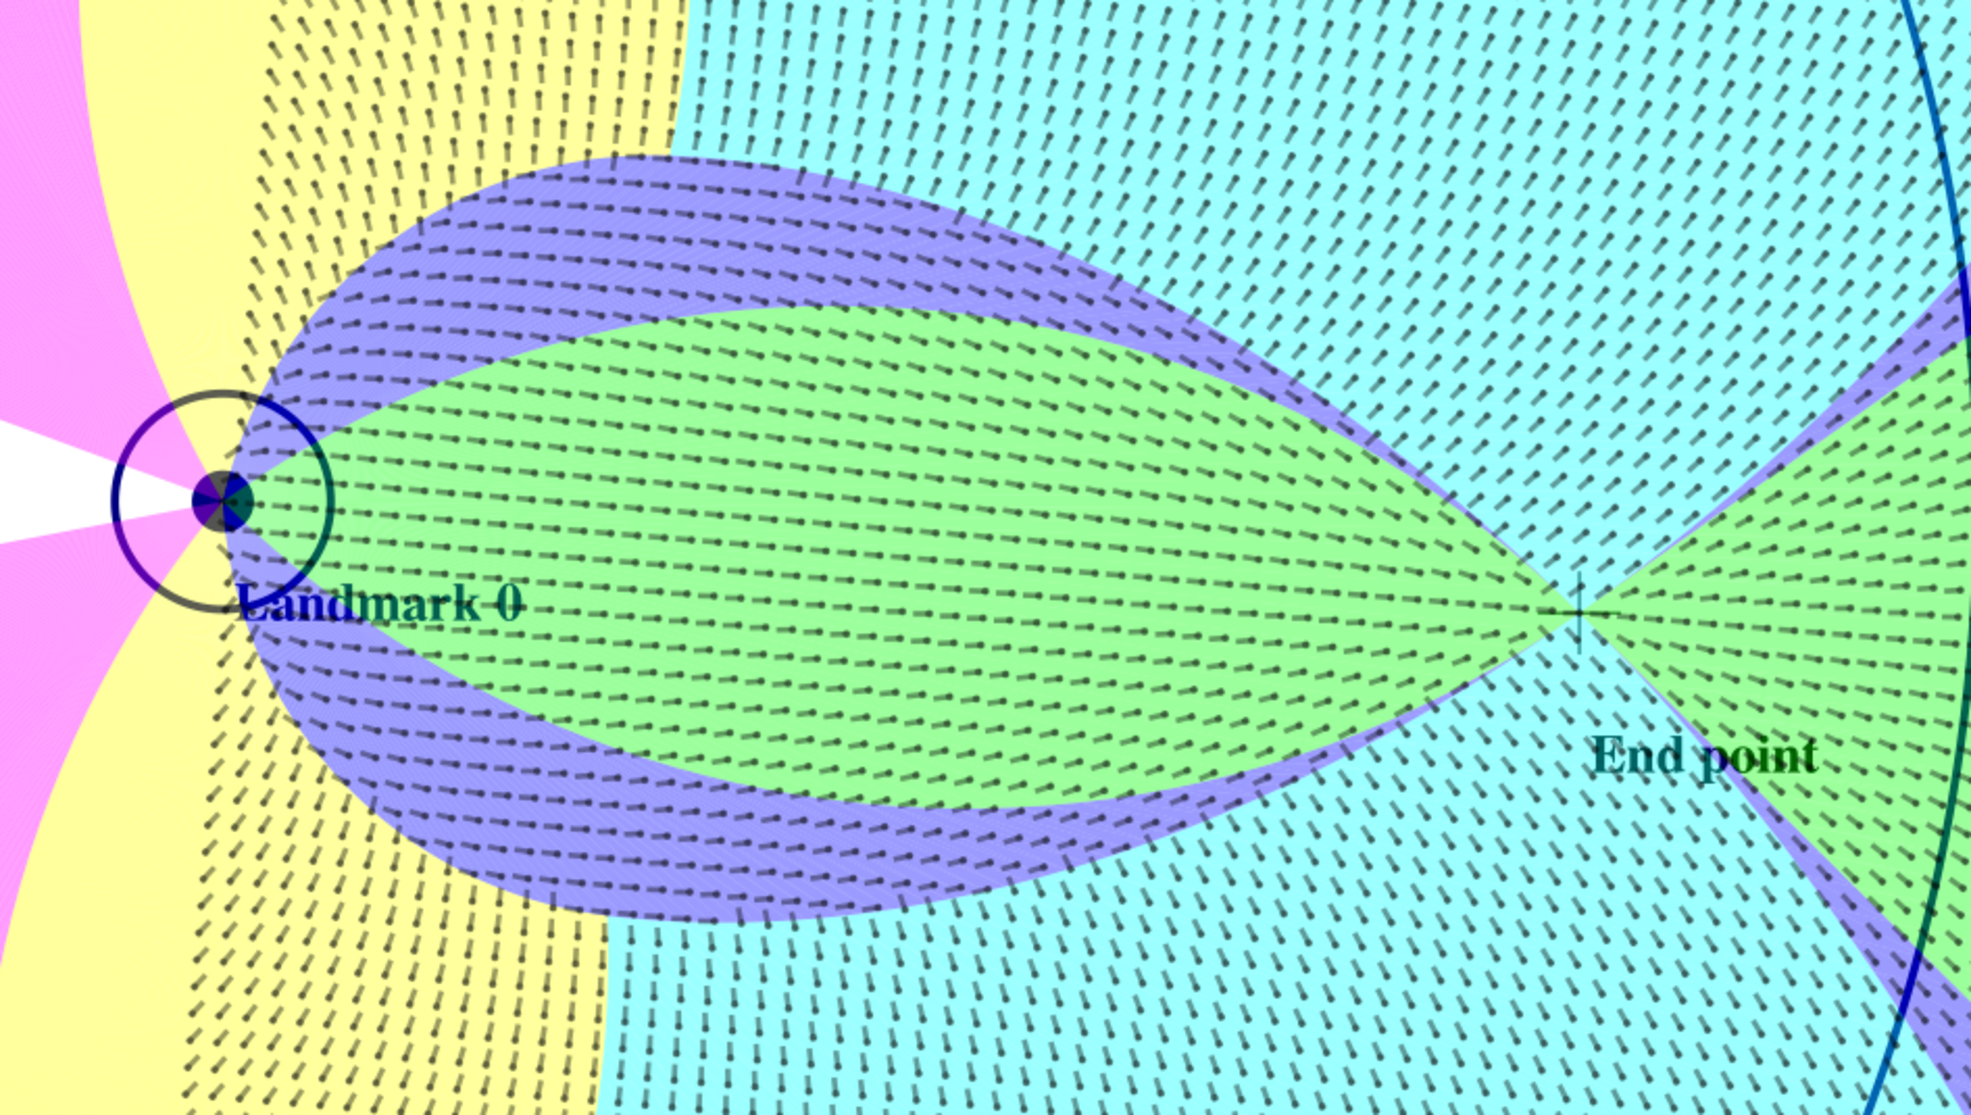
\includegraphics[scale=0.35]{Chap5-Visual-Planning/noLateral}
   \label{fig:fieldNoLateral}
   }
   %\hspace{15 mm}
 \subfigure[Motion direction field with lateral motions.]{
  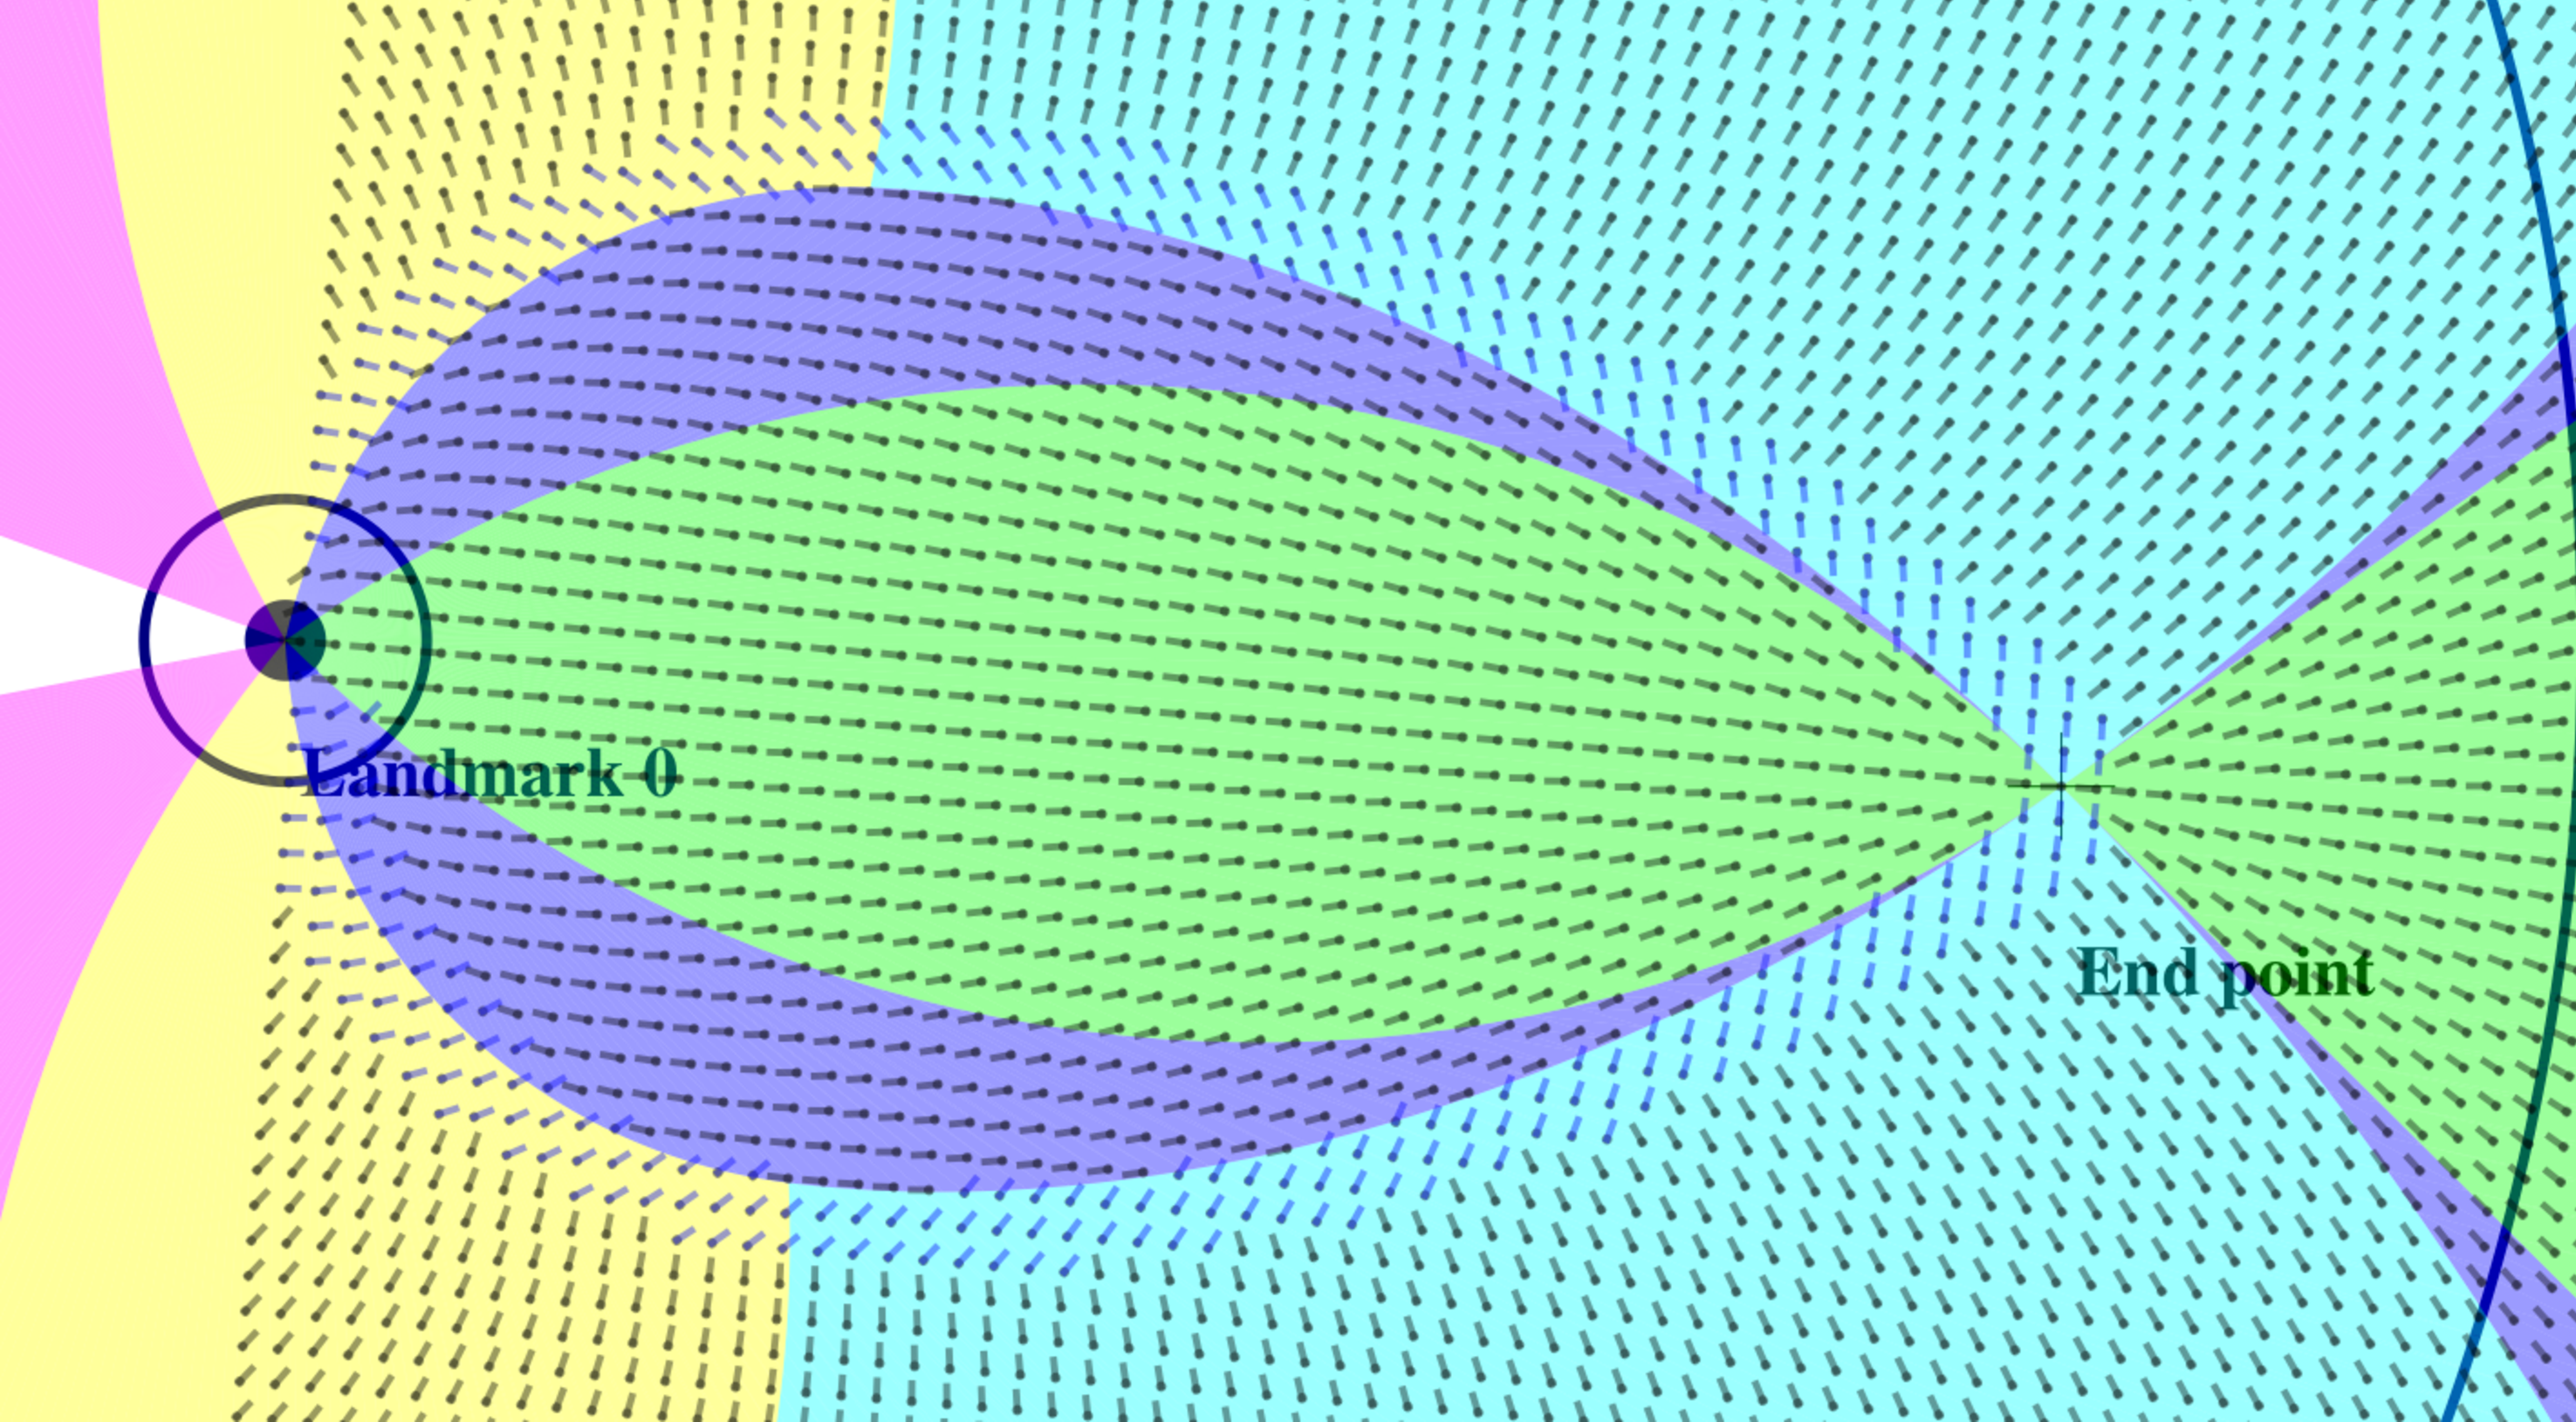
\includegraphics[scale=0.235]{Chap5-Visual-Planning/useLateral}
   \label{fig:fieldUseLateral}
   }
 \caption[]{Visualization of optimal motion directions $\theta^*(x,y)$. Both figures indicate the nature of optimal paths with the filling colors, and the tangent direction to the optimal curve all over a grid defined around the final point. In Fig.~\subref{fig:fieldNoLateral}, the field is computed directly from the primitives of~\cite{Salaris:2010}. The locus of in-site rotations is identifiable at the dark blue zone border. In Fig.~\subref{fig:fieldUseLateral}, the non-holonomy behavior close to this locus is replaced by lateral motions.\label{fig:field}}
\end{figure*}

\subsection{Using the optimal path synthesis within the MPC}

Instead of utilizing in the Equation~\ref{Eq:MinJerk}, a single, constant reference trajectory, defined by the plan computed from $p^s$ to $q^s$, and from which $(\dot{X}_{k+1}^{ref},\dot{Y}_{k+1}^{ref})$ would be evaluated, our idea is to use explicitly the mapping $\sigma$ described above. This way, we can adapt the path execution and find the shortest path to the next sub-goal from any point, not just from $p^s$. As explained above, one can  associate to any $x,y$ the tangent $\theta^*(x,y)$ to the shortest path. One way to enforce the tracking of these shortest paths is to set as a reference velocity (supposing we are following a piece of curve with $v=1$) defined in the time horizon ($l>k$, where $k$ is the current time index):

$$
\begin{array}{ccc}
\dot{x}^{ref}_l =  \cos(\theta^*(x_l,y_l)) & \; & \dot{y}^{ref}_l =  \sin(\theta^*(x_l,y_l)) \\
\end{array}
$$

that depends (non-linearly) on $x_l,y_l$. The idea is to use these -- variable -- reference velocities inside the terms of the pattern generator QP. However, as this mapping is non-linear, a direct use would make us lose the QP form, that allows an efficient resolution of the problem. Because the mapping $\theta^*(x,y)$ has not always an analytic form we evaluate it numerically on a fine scale grid inside the zone of operation of the robot, as pre-computed values, and we also estimate numerically the partial derivatives $\frac{\partial \theta^*(x,y)}{\partial x},  \frac{\partial \theta^*(x,y)}{\partial y}$.

This way, we can approximate each of these reference velocities, at time position $l$ within the optimization time window, by performing a linearization of $\theta^*$  around a reference position $(x^0,y^0)$, i.e.,
$$
\begin{array}{ccc}
\theta^*(x_l,y_l) & \approx & \theta^*(x^0_l,y^0_l)  \\
& & + \frac{\partial \theta^*(x^0,y^0)}{\partial x} (x_l-x^0) + \frac{\partial \theta^*(x^0,y^0)}{\partial y} (y_l-y^0).
\end{array}
$$

Note that the linearization point $(x^0,y^0)$ is chosen in the aforementioned grid of pre-computed values $(\theta^*(x,y),\frac{\partial \theta^*(x,y)}{\partial x},  \frac{\partial \theta^*(x,y)}{\partial y})$, at the closest point to the first (current) CoM position. This grid is depicted in the background of Figs.~\ref{fig:steps6}, \ref{fig:field}, \ref{fig:steps10} among others. To simplify the notation, let us write
$$
\theta^0 \stackrel{\mbox{\tiny def}}{=}  \theta^*(x^0,y^0),\;
\frac{\partial \theta^0}{\partial x} \stackrel{\mbox{\tiny def}}{=} \frac{\partial \theta^*(x^0,y^0)}{\partial x},\;
\frac{\partial \theta^0}{\partial y} \stackrel{\mbox{\tiny def}}{=}  \frac{\partial \theta^*(x^0,y^0)}{\partial y}. 
$$


Then, we re-write the errors to the reference velocities at each time step $l>k$, as a linear function of $\dot{x}_l,\dot{y}_l,x_l,y_l$
$$
\left\{
\begin{array}{ccc}
\dot{x}_l-\dot{x}^{ref}_l & = & \dot{x}_l - v\cos(\theta^0)\\
&& + v\sin(\theta^0) \frac{\partial \theta^0}{\partial x}  (x_l-x^0)\\
&& + v\sin(\theta^0) \frac{\partial \theta^0}{\partial y}  (y_l-y^0),\\
\dot{y}_l-\dot{y}^{ref}_l & = & \dot{y}_l - v\sin(\theta^0_l)\\
&& - v\cos(\theta^0) \frac{\partial \theta^0}{\partial x}  (x_l-x^0)\\
&& - v\cos(\theta^0) \frac{\partial \theta^0}{\partial y}  (y_l-y^0),
\end{array}
\right.
$$ 

and by stacking the errors within the horizon window as in Eq.~\ref{Eq:PosCMHorizon}, we get the following 
linear relations

\begin{eqnarray}
\nonumber
 \dot{C}_{k+1}^{x}  - \dot{X}_{k+1}^{ref} & = &    \dot{C}_{k+1}^{x} -   \dot{C}_{k+1}^{0,x}  + A^x_{0} C_{k+1}^{x}  + B^x_{0} C_{k+1}^{y},\\
 \dot{C}_{k+1}^{y} - \dot{Y}_{k+1}^{ref} & = &   \ \dot{C}_{k+1}^{y} - \dot{C}_{k+1}^{0,y} + A^y_{0} C_{k+1}^{x} + B^y_{0}  C_{k+1}^{y},
 \label{eq-velref-linear}
 \end{eqnarray}

where $A^x_{0},B^x_{0},A^y_{0},B^y_{0}$ are diagonal matrices collecting the terms $v\sin(\theta^0_l) \frac{\partial \theta^0_l}{\partial x}$ and alike. Then, the walking pattern generation is formulated exactly as in Eq.~\ref{Eq:MinJerk}, with the reference velocities given by Eq.~\ref{eq-velref-linear}, and with the optimization variable being $U_{k}$,
%$U_{k} \stackrel{\mbox{\tiny def}}{=}  \left( (\dddot{C}_k^{x})^ \transpose, (X_{k}^{f})^ \transpose, (\dddot{C}_k^{y})^ \transpose, (Y_{k}^{f})^ \transpose \right)^{\transpose}$ 
leading to a canonical Quadratic Program (QP) similar to Eq.~\ref{Eq:QP}.

%{\scriptsize
%\begin{eqnarray}
%\nonumber
% \min\limits_{\dddot{C}^x_k,Z^x_{k+1},\dddot{C}^y_k,Z^y_{k+1}}  &&  \dfrac{\beta}{2} \left\| \dot{C}_{k+1}^{x}  - \dot{X}_{k+1}^{ref} \right\|^2 + \dfrac{\beta}{2} \left\| \dot{C}_{k+1}^{y}  - \dot{Y}_{k+1}^{ref} \right\|^2 \\
%\nonumber
%&& + \dfrac{\gamma}{2} \left\| Z^{x_{ref}}_{k+1} - Z^x_{k+1} \right\|^2 + \dfrac{\gamma}{2} \left\| Z^{y_{ref}}_{k+1} - Z^y_{k+1} \right\|^2 \\
%&& + \dfrac{\alpha}{2} \left\| \dddot{C}_{k}^{x}  \right\|^2 + \dfrac{\alpha}{2} \left\| \dddot{C}_{k}^{y} \right\|^2,
%\label{eq-main-qp}
%\end{eqnarray}
%}

% that can be expressed in terms of $U_{k} \stackrel{\mbox{\tiny def}}{=} \left( (\dddot{C}_k^{x})^ \transpose, (Z_{k+1}^{x_{ref}})^ \transpose, (\dddot{C}_k^{y})^ \transpose, (Z_{k+1}^{y_{ref}})^ \transpose \right)^{\transpose}$ by using Eq.~\ref{eq-velref-linear}, into a canonical Quadratic Program (QP) similar to Eq.~\ref{Eq:QP}.

The constraints arising from the CoP position to be included in the support polygon being non-linear in the feet orientation, we simply set the robot and feet orientations as follows and include the computed values into the QP.

\subsection{Control of the rotation angle}
In order for the robot to be oriented with the tangent to the optimal path, $\theta^0$, and to keep the QP form, we use a decoupled approach for the control of the rotation angles of the CoM and the feet~\cite{HerdtIROS2010}. Hence, in a first stage, we optimize the orientations in the MPC time window by  

\begin{eqnarray}
\nonumber
 \min\limits_{\dddot{C}_k^{\theta},\dddot{F}_k^{\theta}}  &&  \dfrac{\beta}{2} \left\| C_{k+1}^{\theta} - \theta^{0} \right\|^2 + \dfrac{\gamma}{2} \left\| F_{k+1}^{\theta} - \theta^{0} \right\|^2 \\
\nonumber && + \dfrac{\alpha}{2} \left\| \dddot{C}_{k}^{\theta} \right\|^2 + \dfrac{\alpha}{2} \left\| \dddot{F}_{k}^{\theta} \right\|^2,
\end{eqnarray}

and then in a second stage, we introduce these angles as constant in the main QP (Eq.~\ref{Eq:MinJerk}). This approach gives us the advantage of introducing constraints like maximum rotation between both feet, between feet and trunk and also a rotation limit to keep the visibility of the landmarks.

%\subsection{Refinement of the angular position}

%\textcolor{blue}{JB:} Will we do something about that?: the idea would be to do a second pass where the $\theta^0$ would be re-evaluated.

%\textcolor{blue}{MG:} You meant the linearization points right, is it still necesary after the clarification?

%=============================================================================================================================================================

\section{Including holonomic behavior}
\label{sec:includingholonomic}

Handling holonomic and non-holonomic behaviors together during locomotion has been previously been discussed in \cite{MombaurHumanoids2008} in a context of motion planning.

One of the most visible disadvantages of the optimal non-holonomic paths given from~\cite{jib-IJHR2010} is the presence of in-site rotations, that are not efficient in terms of footsteps number.
One solution is to use a different formulation of the cost function using weights according to the robot direction and control the head.
But including this vision based control in Eq.~\ref{Eq:MinJerk} is incompatible with a QP formulation.
A strategy we propose here is to take advantage of the fact that the set of points where in-site rotations occur is very well defined geometrically in the plane, as a direct consequence of the synthesis from~\cite{Salaris:2010}. As illustrated in Fig.~\ref{fig:fieldNoLateral}, it is the outer boundary of the partition zone where the shortest paths have to be done as line segments followed by spirals, i.e. the dark blue region of the figure. This curve is made of two parts~\cite{Salaris:2010}, one arc of circle and one piece of logarithmic spiral. Hence, we propose to perform the following: for all points inside the partition regions in contact with this locus, we evaluate its distance in terms of the primitive to be done to reach this locus and modify the reference velocities as follows. 

If the robot is far from the locus of in-site rotations, then the path to follow is continuously derivable and goes either forwards or backwards; in that case, we use the ``non-holonomic behavior'' as described in Section~\ref{sec:reftrajectories}, with the robot orientation controlled to stay close to $\theta^*(x_l,y_l)$,
$$
\begin{array}{c}
\dot{x}^{ref}_l  =  \cos(\theta^*(x_l,y_l)) \;,\; \dot{y}^{ref}_l  =  \sin(\theta^*(x_l,y_l)), \\
\end{array}
$$

and if the robot configuration is close to this locus, then we use instead lateral motions, with orientation $\phi(x_l,y_l)+\pi$, where $\phi(x_l,y_l)=\arctan\frac{y_l}{x_l}$ is the polar angle of $(x_l,y_l)$,
$$
\begin{array}{c}
\dot{x}^{ref}_l  =  -\varepsilon\sin(\phi(x_l,y_l)) \;,\; \dot{y}^{ref}_l  =  \varepsilon\cos(\phi(x_l,y_l)),  \\
\end{array}
$$

where $\varepsilon =\pm1$ in function of the relative position of the goal to reach with respect to the evaluated point. 

In Fig.~\ref{fig:fieldUseLateral}, we illustrate this modification by drawing the lateral motion field with blue arrows, together with the ``non holonomic'' field ``far'' from the locus of in-site rotations. 

%=============================================================================================================================================================
\section{Results}
\label{sec:results}

%=============================================================================================================================================================

In this section, we present three experiments. In the first one, we test the performance of our approach in the absence of localization uncertainty, and with only non-holonomic motion. In the second one, we introduce localization uncertainty. In the last one, we present an improvement to the border behavior with the possibility of holonomic motion. The three experiments have the same set-up, with initial position in $(0.5,2.5)$, landmark position in $(0,0)$ and final position in $(-3,0)$. We chose this trajectory because it makes the robot pass through several regions of the partition and illustrates the border behavior which is one of the problems we found.

In Fig.~\ref{fig:steps6}, we depict the performance in perfect and noiseless conditions. We see that using the planner vector field for driving the robot to the goal produces smooth and stable trajectories of the CoM. However, in real conditions, the robot will not perform the control exactly e.g., because of sliding with the floor. Moreover the robot needs a localization system which will be inherently noisy. To model this situation we perturbed the current position of the CoM with white gaussian noise $\sim \mathcal{N}(0,\sigma^2)$ in each coordinate with $\sigma = 0.2$ and with $\sigma = 10$ degrees for the orientation.

\begin{figure}[ht]
\centering
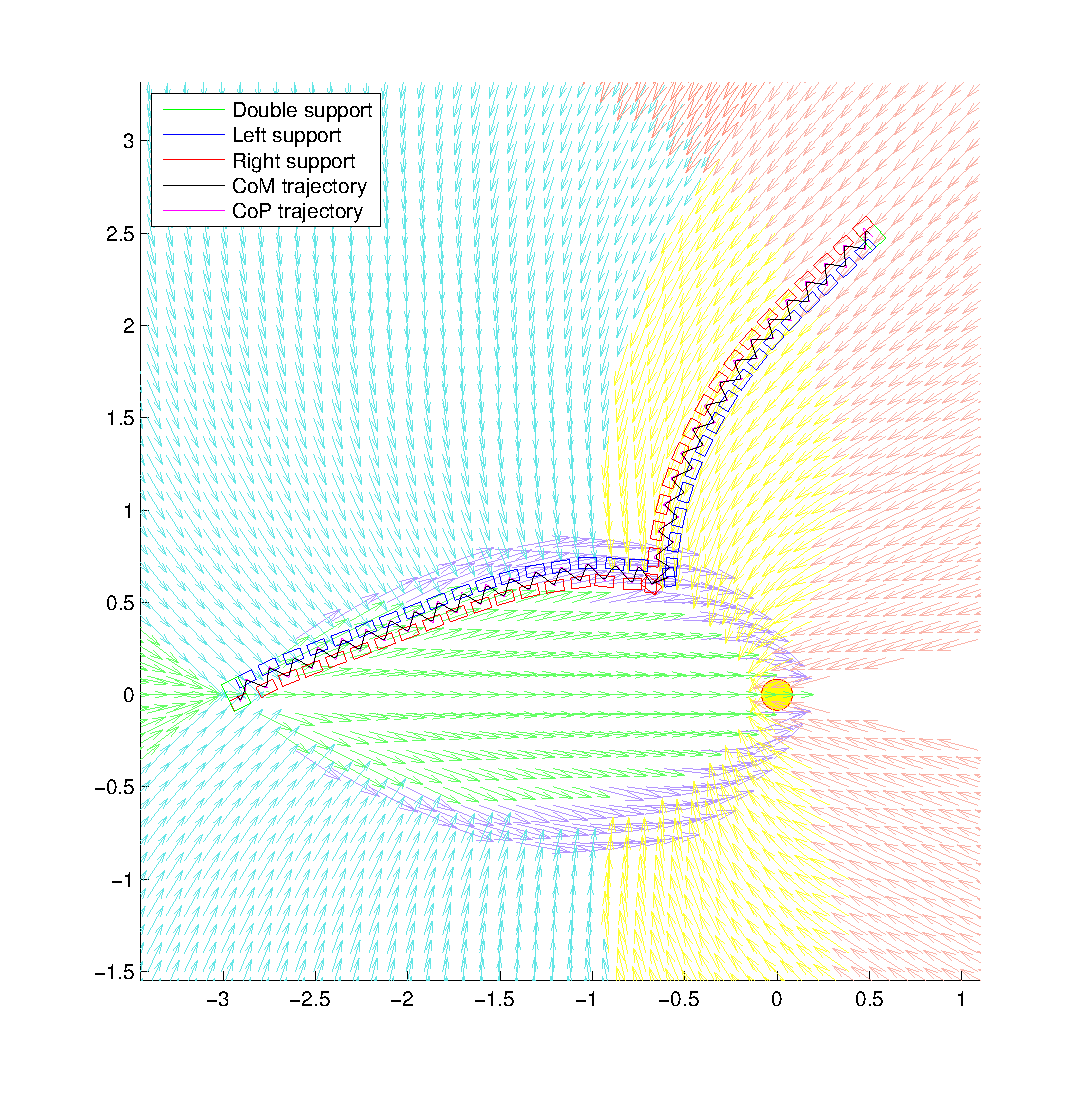
\includegraphics[scale=0.8]{Chap5-Visual-Planning/steps6.pdf}
\caption{Vector fields generated by optimal trajectories planned with visibility constraints for a non-holonomic robot~\cite{Salaris:2010}. To each color is associated a family of global paths that reach the goal (at $(-3,0)$) according to the current configuration of the robot while keeping the landmark (yellow disk) visible at all times. The footsteps, CoM and CoP trajectories for the humanoid robot are all depicted as indicated in the upper box.}
\label{fig:steps6}
\end{figure}

In Fig. \ref{fig:steps10}, we show the behavior in that situation. We can still appreciate a smooth trajectory in the regions far from the border of the dark blue region of the partition, where the vector field is smooth. We also notice the good behavior of the orientation angle mainly because the QP formulation controls it. The main problem of this approach also appears: The discontinuities in the partition regions in which an in-site rotation occurs. Hence, the robot may perform unnecessary maneuvers, involving in-site rotations, which is far from optimal in the case of human walking (Fig.~\ref{fig:steps10zoom}). Moreover, in-site rotations cause high rotation speeds of the feet (Fig.~\ref{fig:velocities10}), which is not desirable from a balance point of view.

\begin{figure}[ht]
\centering
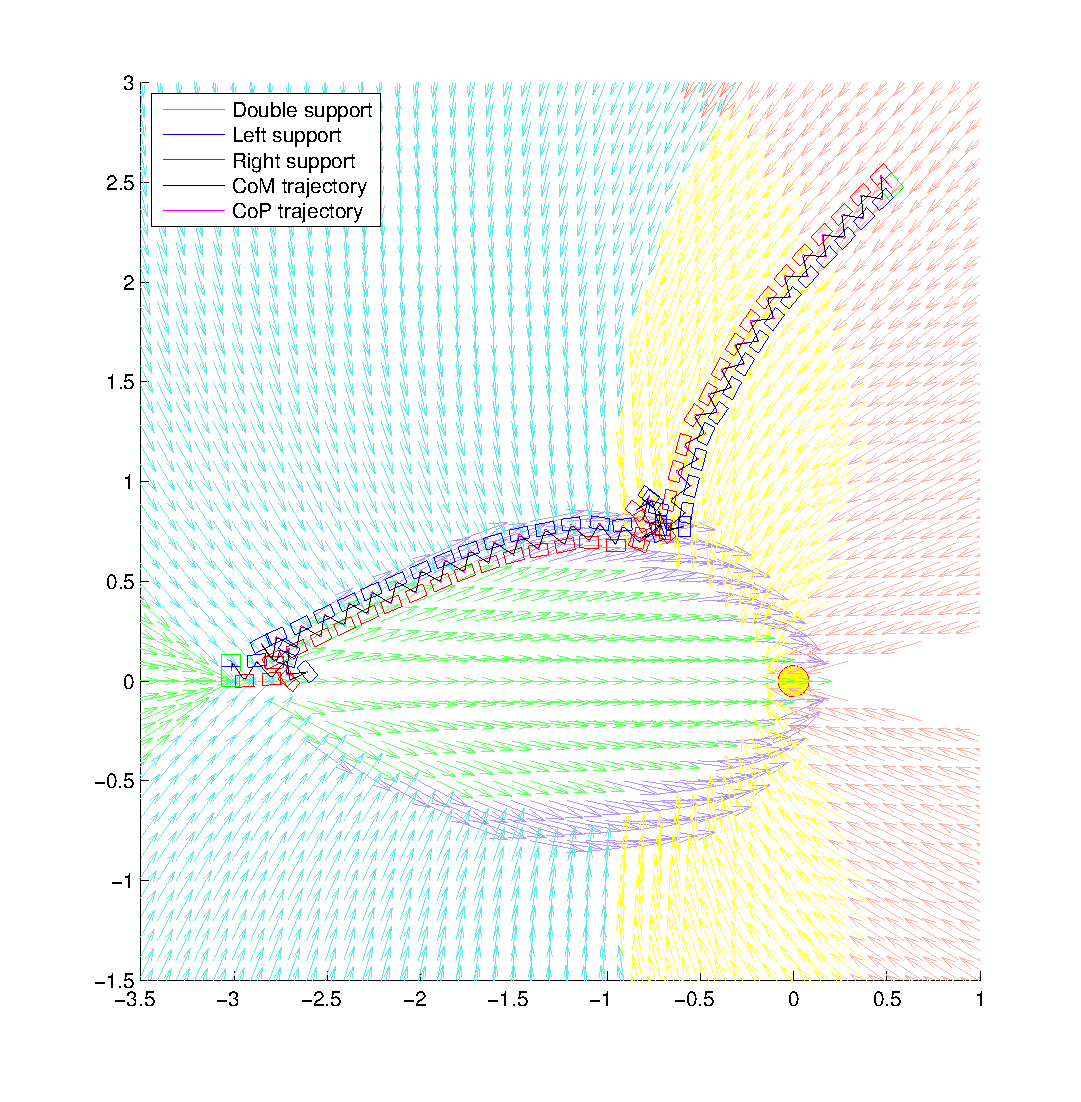
\includegraphics[scale=0.8  ]{Chap5-Visual-Planning/steps10.pdf}
\caption{If the control is not followed well and if we use an imperfect localization system, problems may arise in the borders of the partition, in case of relying on purely non-holonomic behaviors.}
\label{fig:steps10}
\end{figure}

\begin{figure}[ht]
\centering
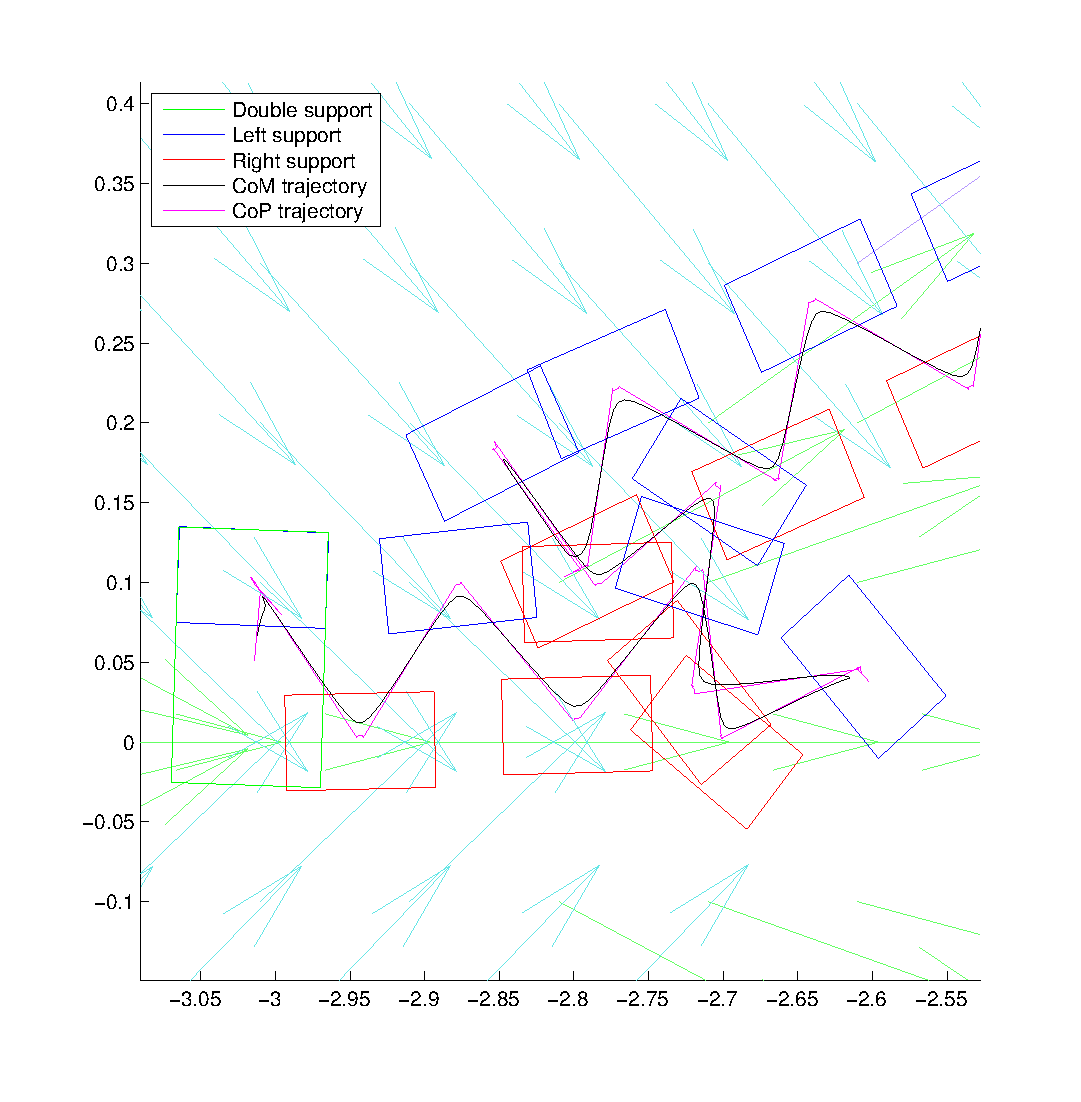
\includegraphics[scale=0.55]{Chap5-Visual-Planning/steps10zoom.pdf}
\caption{Zoom on Fig.~\ref{fig:steps10}, close to $(-3,0)$. As the robot compensates sliding and localization errors non-holonomically, more in-site rotations occur.}
\label{fig:steps10zoom}
\end{figure}

\begin{figure}[ht]
\centering
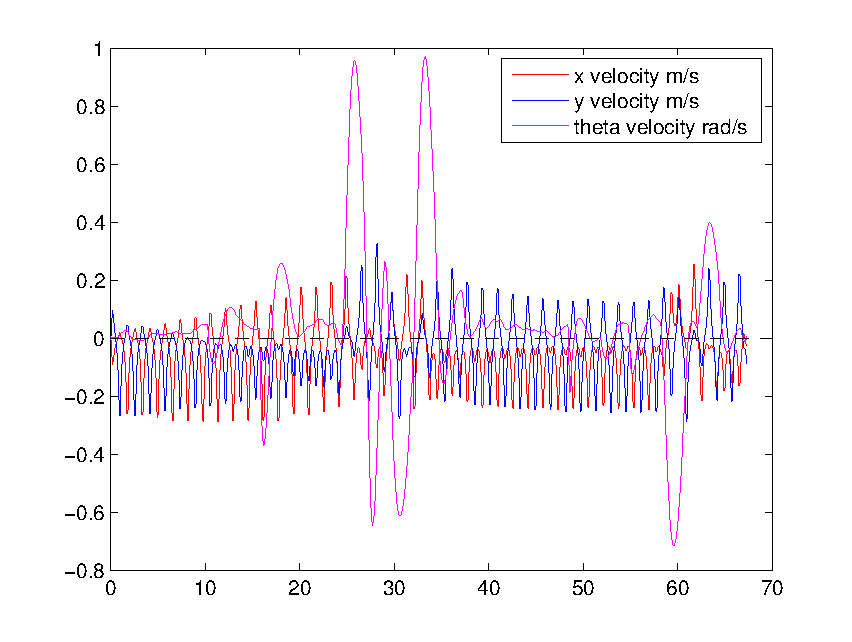
\includegraphics[scale=0.7  ]{Chap5-Visual-Planning/velocities10.pdf}
\caption{Velocities profile for the trajectory depicted in Fig.~\ref{fig:steps10}. The overshoots in the angular velocity are caused by the in-site rotations at the border of the dark blue region of the partition.}
\label{fig:velocities10}
\end{figure}

To address the aforementioned problem, we present the results of the improvement introduced in Section~\ref{sec:includingholonomic}. In Fig.~\ref{fig:steps11}, we perform the same trajectory but by introducing the possibility of holonomic motion in the region where in-site rotations would be necessary. The robot is not performing in-site rotations anymore, but a mixture of holonomic and non-holonomic motions, depending on its position with respect to the border. We can appreciate better the transition between non-holonomic and holonomic motions in Fig. \ref{fig:steps11zoom}. %Finally in Fig. \ref{fig:velocities11} we can see the reduction of the angular velocity necesay to perform the motion.

\begin{figure}[ht]
\centering
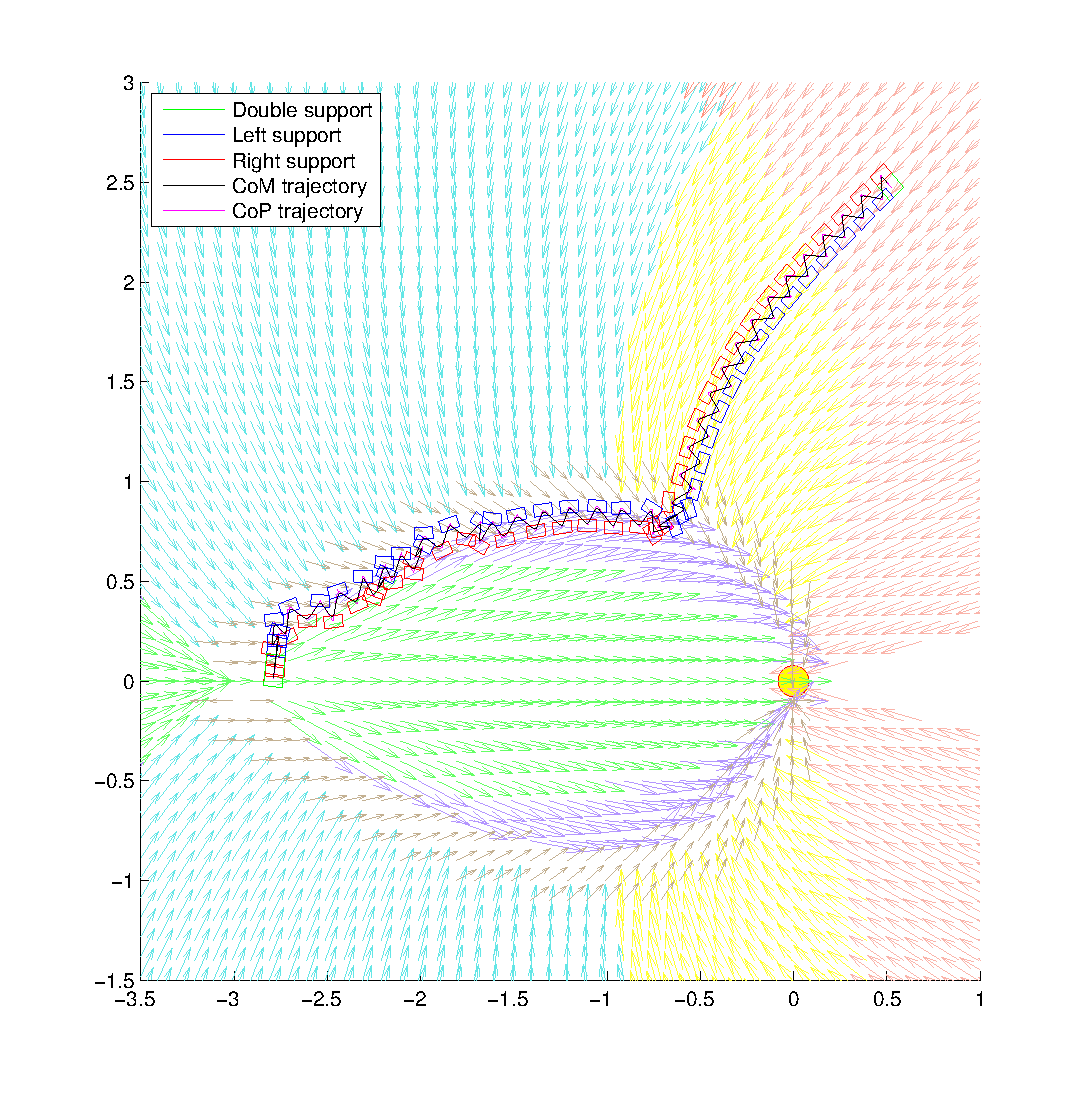
\includegraphics[scale=0.8  ]{Chap5-Visual-Planning/steps11.pdf}
\caption{Trajectory with holonomic motion made possible. Lateral motion is allowed in the khaki vector field in the orientation discontinuity region.}
\label{fig:steps11}
\end{figure}

\begin{figure}[ht]
\centering
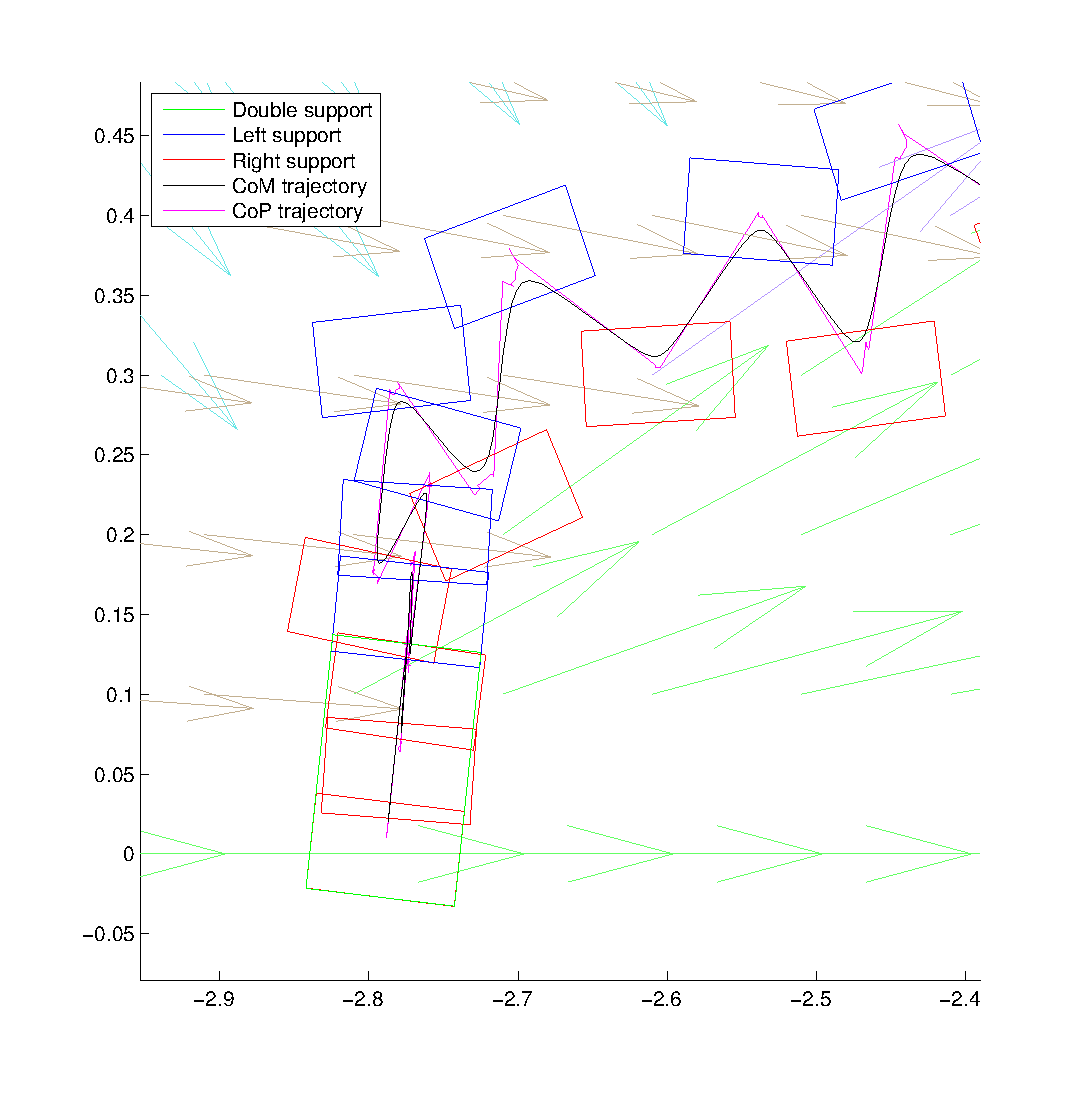
\includegraphics[scale=0.55]{Chap5-Visual-Planning/steps11zoom.pdf}
\caption{Transition between non-holonomic and holonomic controls. Moving sideways is much more efficient for such a trajectory to the goal.}
\label{fig:steps11zoom}
\end{figure}

%\begin{figure}
%\centering
%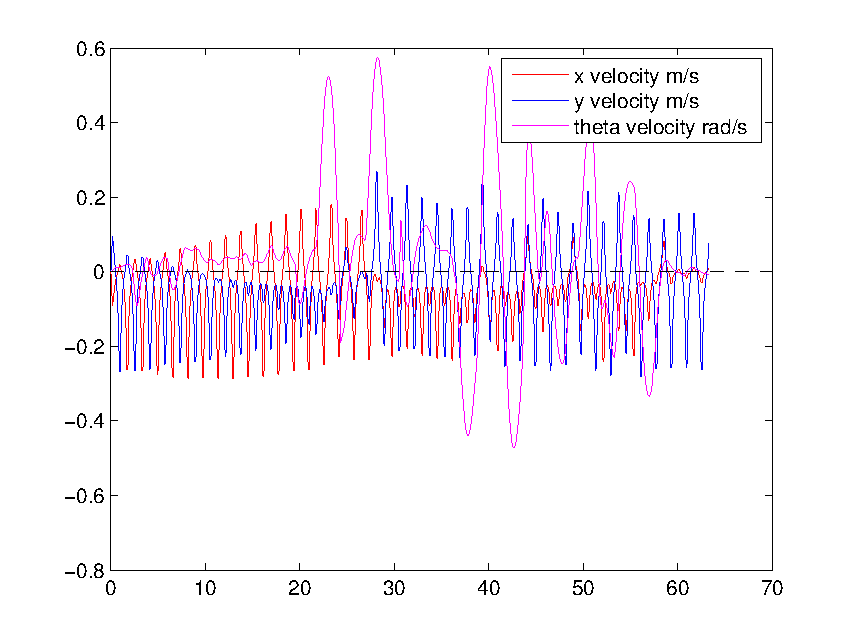
\includegraphics[scale=0.4]{velocities11.pdf}
%\caption{Velocities profile for the trajectory of the figure \ref{fig:steps11}. We can see that those velocities are in good limits and provide a stable walking. }
%\label{fig:velocities11}
%\end{figure}

%=============================================================================================================================================================
\section{Conclusion}
\label{sec:conclusion}
%=============================================================================================================================================================

In most of the current literature, the link between planning and locomotion control has been given by footsteps. In this paper, we propose a novel approach that uses directly the optimal motion synthesis derived from the planner to the control system without going through footsteps but instead by computing them within the Walking Pattern Generator. With this approach, we can drive the robot to a desired goal by using an external planner, not necessarily the one used in this paper. We tested our approach simulating real situations such a localization noise. We have also tried to make the walking pattern more efficient by introducing the possibility of using holonomic motion. Our next objective is to test the approach introduced in this paper on the HRP-2 platform.
